%%%%%%%%%%%%%%%%%%%%%%%%%%%%%%%%%%%%%%%%%%
% Master Thesis 
% Polina Polunina
% October 2022 
%
% License:
% CC-BY-SA 4.0 -- Creative Commons Attribution-ShareAlike 4.0 International
% https://creativecommons.org/licenses/by-sa/4.0/legalcode
%%%%%%%%%%%%%%%%%%%%%%%%%%%%%%%%%%%%%%%%%%
\section{Appendix} \label{sec:apendix}
    \subsection{Listings}
\begin{lstlisting}[language=python, caption=python script to, label=list:methods:freyja-s1]
 Sample name	summarized	lineages	abundances	resid	coverage
 sample1 	[('Omicron', 0.6999889999983451), ('Delta', 0.22408099987442534), ('Other', 0.07552100018490182)]	BA.1.18 AY.4 BA.1.19 BA.1.1.13 BA.1.15.1 AY.38 BA.1.9 BA.1.16 B B.1.617.2 B.1.1.529 XS	0.23943700 0.11764700 0.11363600 0.10000000 0.09667000 0.06944400 0.06686400 0.06474800 0.06122400 0.03699000 0.01863400 0.01429700	7.611495978	99.95971667
\end{lstlisting}
    \subsection{Further figures}
        \subsubsection{Existing Galaxy workflows that were not changed} \label{sec:appendix:figures:wfs}
        Other existing Galaxy workflows for SARS-CoV-2 clinical data surveillanve that were not taken as a basis for improvement and repurposing in this thesis are presented in \cref{fig:further:ont-wf} and \cref{fig:further:illumina-wf}.
        \begin{landscape}
        \centering\vspace*{\fill}
        \begin{figure}[ht!]
        	\centering
            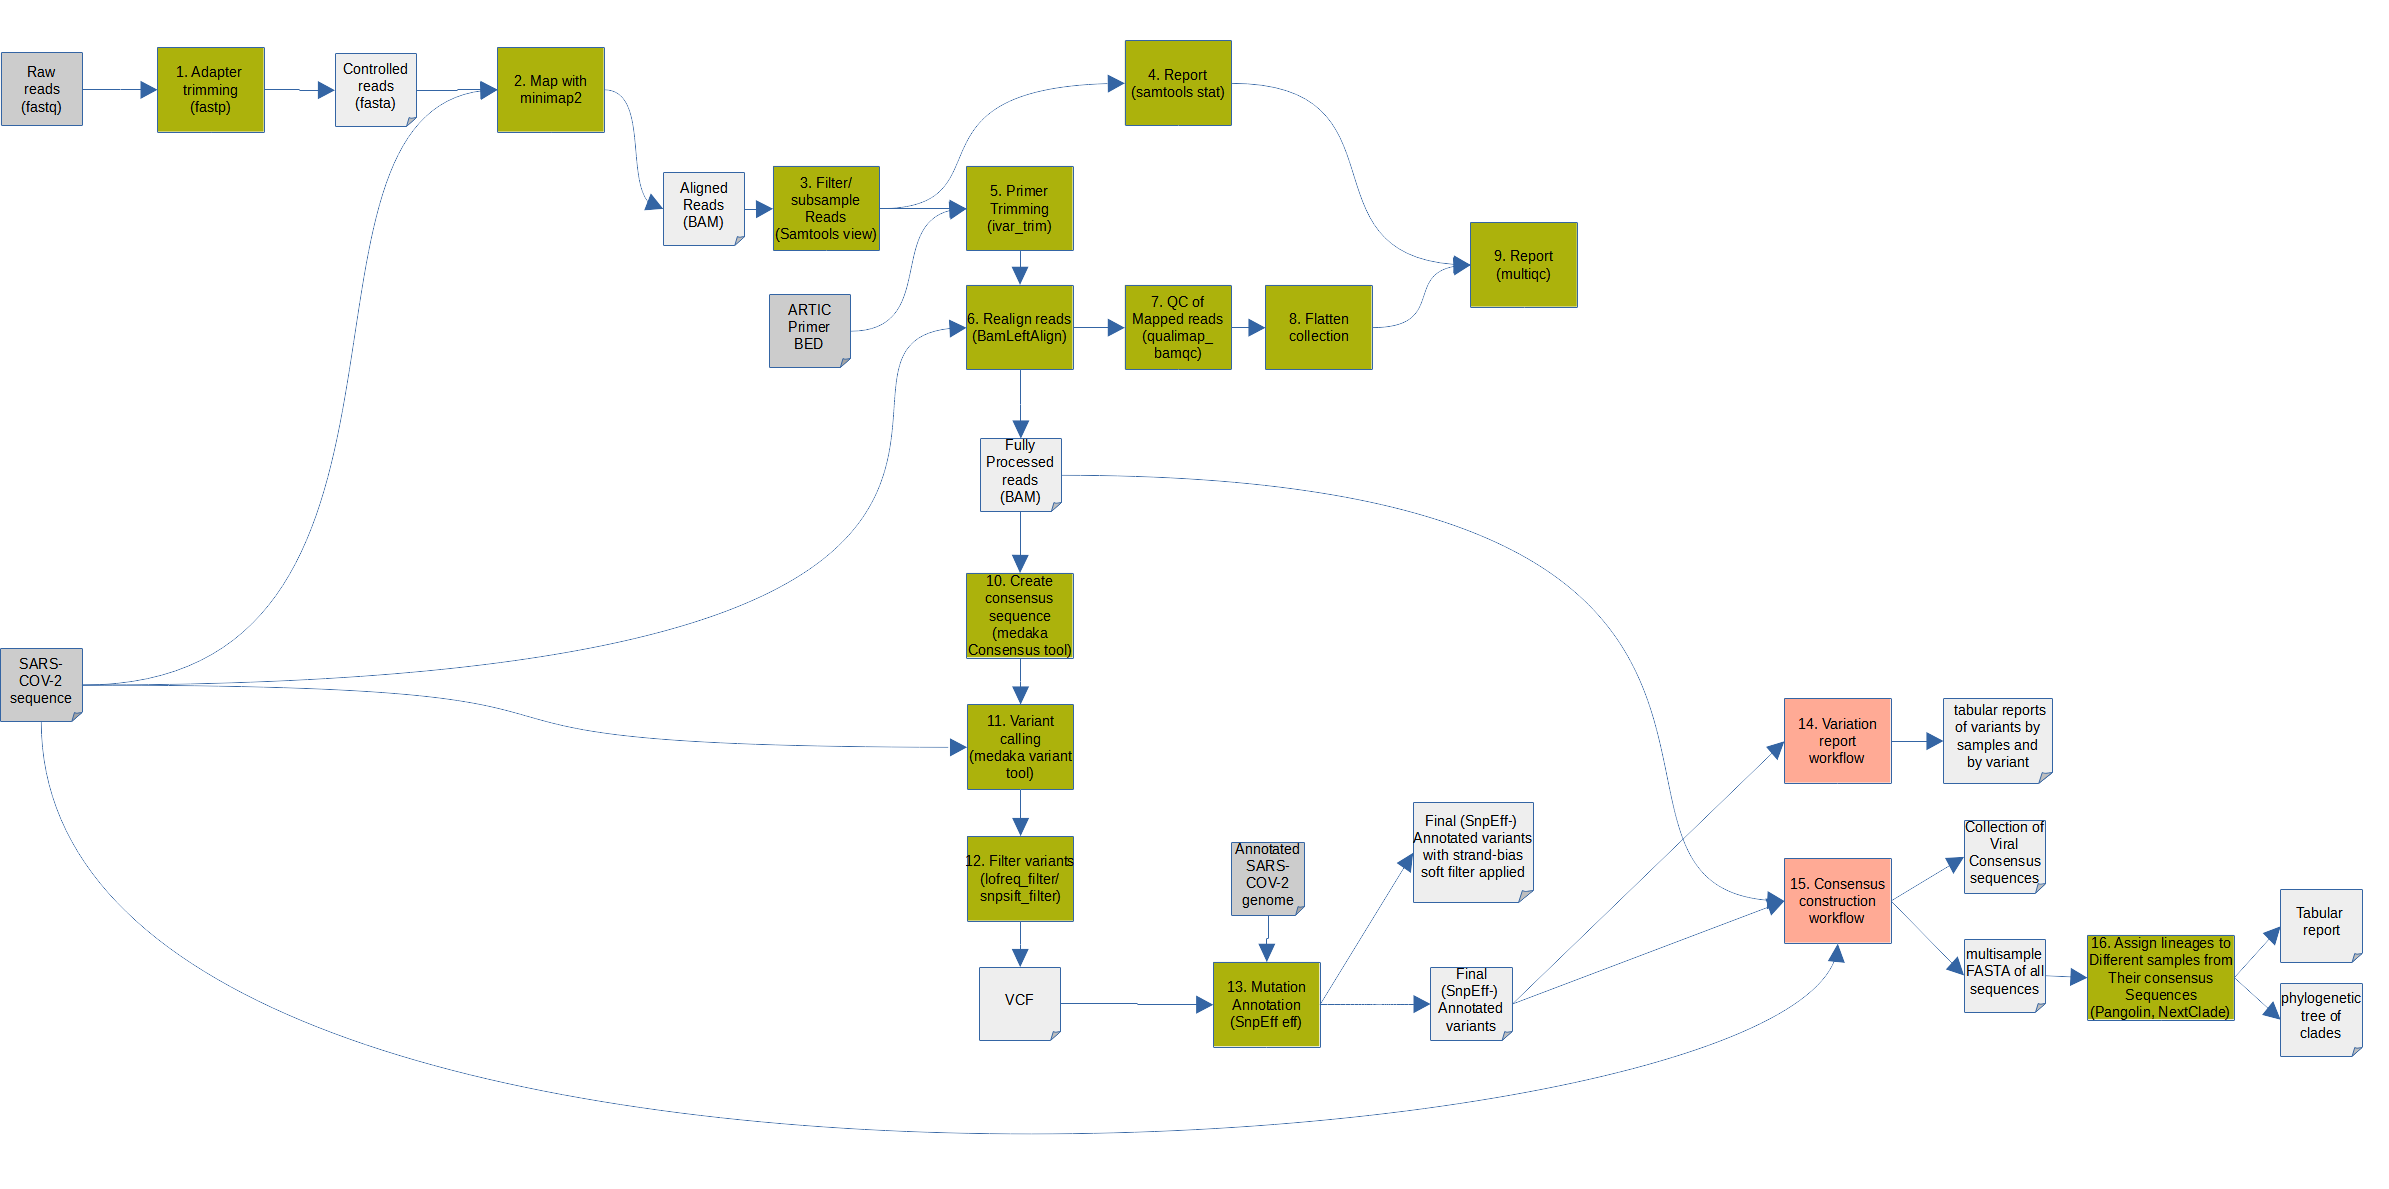
\includegraphics[width=1.4\textwidth]{figures/further/further-ont-wf.png}
            \captionof{figure}{One of four existing Galaxy workflow for SARS-CoV-2 clinical data surveillance for single-end reads data extracted with amplicon-based technique and sequenced with Nanopore sequencing approach.}
            \label{fig:further:ont-wf}
        \end{figure}
        \begin{figure}[ht!]
        	\centering
            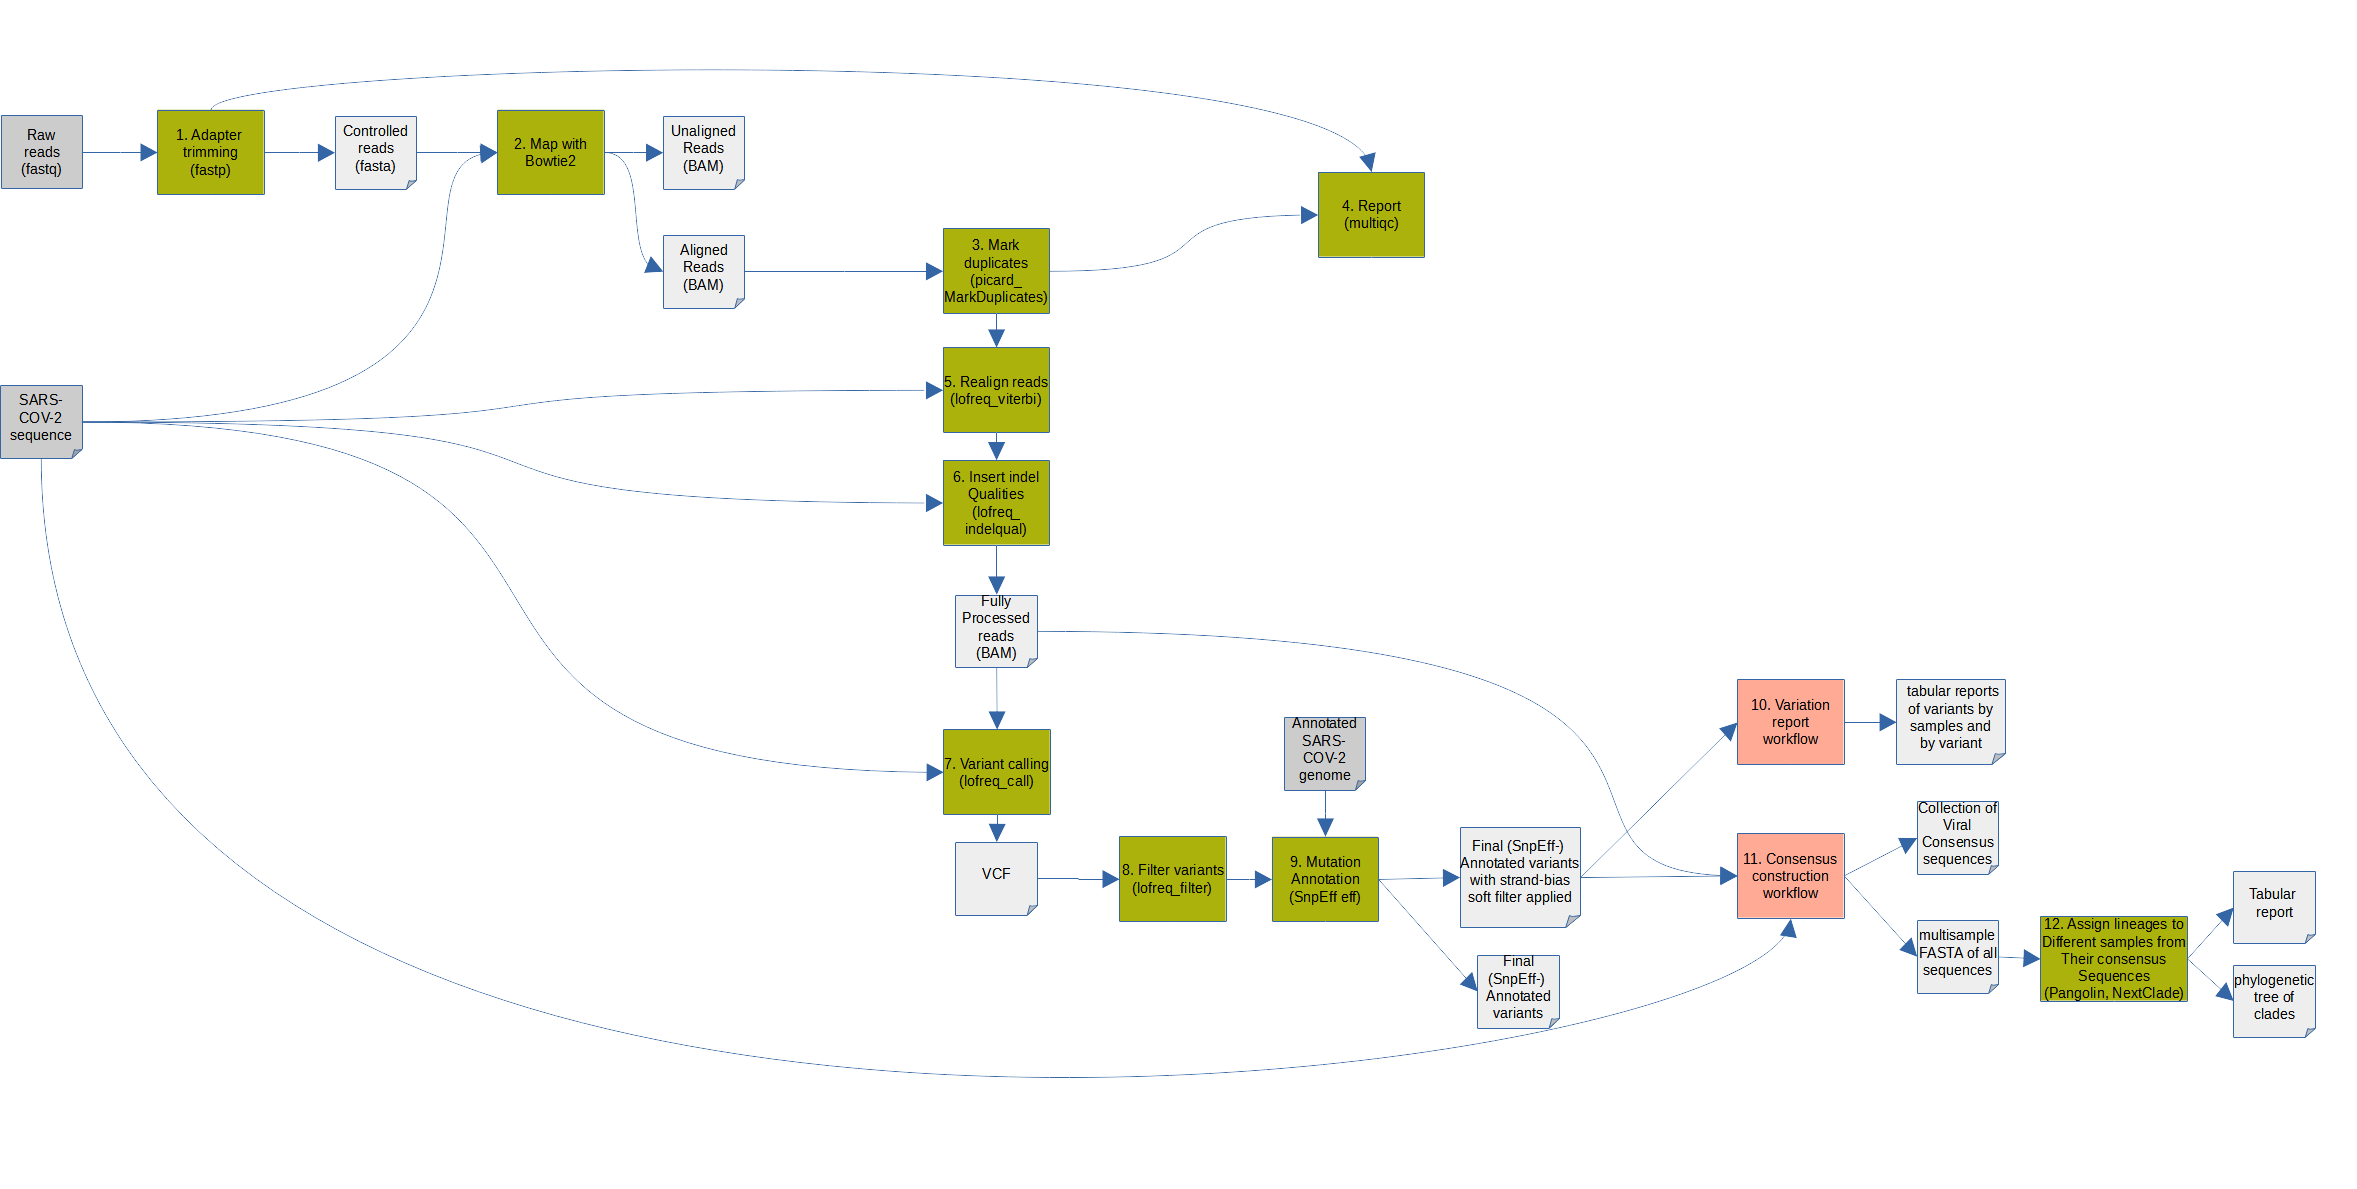
\includegraphics[width=1.4\textwidth]{figures/further/further-illumina-wf.png}
            \captionof{figure}{One of four existing Galaxy workflow for SARS-CoV-2 clinical data surveillance for single-end reads data extracted with metatranscriptomic-based technique and sequenced with Illumina sequencing approach.}
            \label{fig:further:illumina-wf}
        \end{figure}
        \vfill
        \end{landscape}
        
        
\clearpage

